\section{Appendix (System and Raspberry Pi specifications)}
\label{sec:sysetm_specs}

The following setup was used to collect results and benchmarking data:

\begin{table}[htbp]
	\centering
	\begin{tabular}{@{}lccc@{}}
		\toprule
		\textbf{Specification} & \textbf{Desktop} & \textbf{RPI5} & \textbf{RPI4 Model B} \\ 
		\midrule
		Processor             & AMD Ryzen 7 5800H & Cortex A-76 & Cortex A-72 \\
		Processor Type          & x86                      & ARM            & ARM \\
		Processor Speed        & 3.2 - 4.4 GHz       & 2.4 GHz       & 1.5 - 1.8 GHz\\
		Cores/Threads            & 8/16                    & 4/4                & 4/4 \\
		RAM Size                   & 16GB                  & 8GB              & 4GB \\
		RAM Type                  & DDR4                  & LPDDR4       & LPDDR4 \\
		RAM Speed                & 3200 MT/s           & 4267 MT/s    &3200 MT/s \\
		Operating System      & Ubuntu Linux 22.04.4 LTS & Debian Linux 12 (bookworm) &  Debian Linux 12 (bookworm)\\
		GCC Compiler           & 11.4.0               & 12.2.0        &  12.2.0\\
		GNAT Compiler         & 10.5.0               & 12.2.0        &  12.2.0\\
		Java Compiler            & 11.0.22            & 17.0.10      &  17.0.10\\
		C\# (.NET SDK)         & 7.0.117             & 6.8.0.15     &  6.8.0.15\\
		\bottomrule
	\end{tabular}
	\caption{Specifications and software Versions of Desktop and Raspberry Pi Systems\cite{rasp_pi5_pi4_comparision}\cite{desktop_specs}\cite{rpi_specs}.}
	\label{tab:spec_comparisons}
\end{table}

\newpage
\section{Appendix (Objective 1: \texttt{mpbenchmark})}
\label{sec:app_obj1}

Profiling results using \texttt{Valgrind/Calgrind} are shown in figure ~\ref{fig:mpbenchmark_profiled}.

\begin{figure}[H] % Positioning preference: here, top, bottom, page
	\centering
	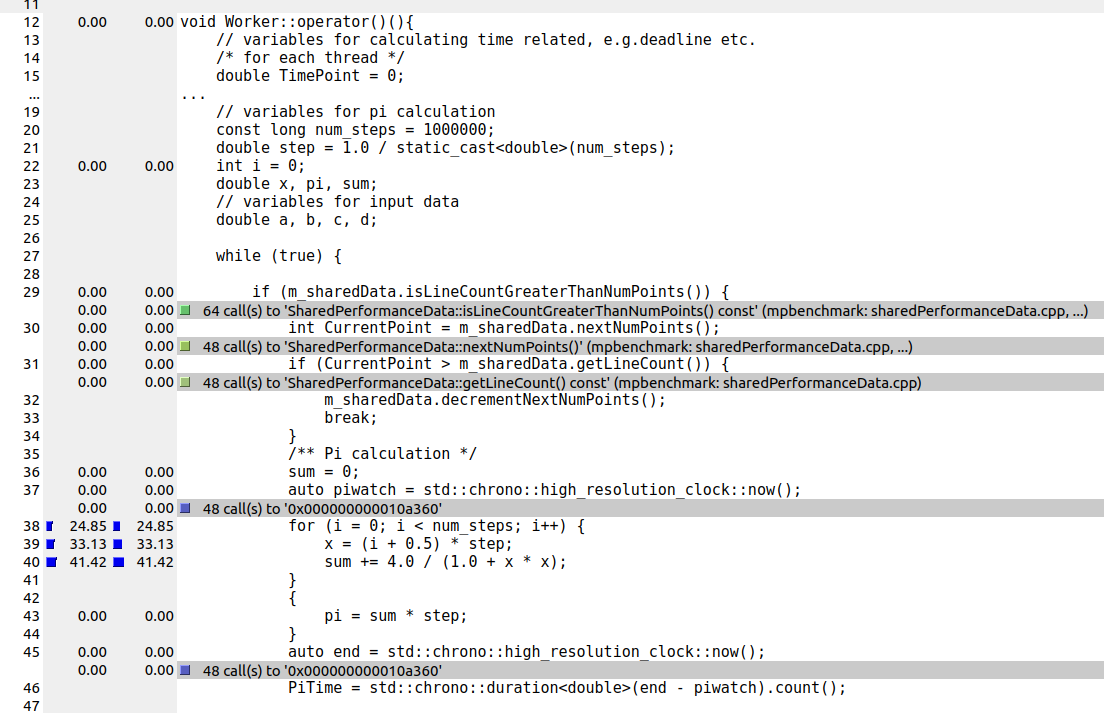
\includegraphics[width=1\textwidth, height=20cm]{~/Documents/Part_D_Modules/Individual_Project/Individual_report/figures/valgrind_mpbenchmark.png} % Adjust the path and width as needed
	\caption{\texttt{Calgrind} profiling results on the \texttt{mpbenchmark} application. Ir - Instruction Fetch, CEst - Cycle estimation.}
	\label{fig:mpbenchmark_profiled} % Use this label to reference the figure
\end{figure} 

Listing ~\ref{lst:avx2_horizontal_sum_function} shows the code for the horizontal sum function for performing the sum of \texttt{256-bit} vector using \texttt{AVX2} instructions. 

\begin{lstlisting}[
	caption={Horizontal sum function for \texttt{256-bit} \texttt{AVX2} vector.},
	label={lst:avx2_horizontal_sum_function}
	]
// Check for AVX2 support
#if defined(__AVX2__)
#include <immintrin.h> // AVX2 and earlier

/**
* @brief Helper function used when approximating pi using AVX2 instructions. 
* It is used for performing horizontal sum of a vector. 
* @param v vector. 
* @return double summed vector.
*/
inline double hsum256_pd(__m256d v) {
	__m256d temp1 = _mm256_hadd_pd(v, v);
	__m256d temp2 = _mm256_permute2f128_pd(temp1, temp1, 0x01);
	__m256d temp3 = _mm256_add_pd(temp1, temp2);
	double result[4];
	_mm256_storeu_pd(result, temp3);
	return result[0]; // The sum of all elements in the vector
}

#elif defined(__ARM_NEON)
// if ARM NEON instructions are available then include the necessary header file 
#include <arm_neon.h>

#else
// neither AVX2 or NEON instructions found 
#endif

\end{lstlisting}

Code for implementing the approximation of $\pi$ using single and double point floating precision with \texttt{NEON} instructions are shown in Listings ~\ref{lst:neon_float} and ~\ref{lst:neon_double}.

\begin{lstlisting}[
	caption={Approximation of $\pi$ using single point precision \texttt{NEON} instructions.},
	label={lst:neon_float}
	]
double Worker::approximatePi(){
	double pi = 0.0;
	static constexpr long num_steps = 1000000;
	static constexpr double step = 1.0 / static_cast<double>(num_steps);
	
	#if defined(__AVX2__)
	// Insert AVX2 specific code here ...

	#elif defined(__ARM_NEON)
	// Insert NEON specific code here
	float32_t f_step = 1.0f / static_cast<float32_t>(num_steps); // Using float for NEON
	float32x4_t vec_step = vdupq_n_f32(f_step);
	float32x4_t vec_half_step = vdupq_n_f32(0.5f * f_step);
	float32x4_t vec_one = vdupq_n_f32(1.0f);
	float32x4_t vec_four = vdupq_n_f32(4.0f);
	float32_t sum = 0.0f; // Using float for NEON
	
	for (int i = 0; i < num_steps; i += 4) {
		float32x4_t vec_i = vsetq_lane_f32(i + 3, vsetq_lane_f32(i + 2, vsetq_lane_f32(i + 1, vsetq_lane_f32(i, vdupq_n_f32(0.0f), 0), 1), 2), 3);
		float32x4_t vec_x = vaddq_f32(vmulq_f32(vec_i, vec_step), vec_half_step);
		float32x4_t vec_temp = vdivq_f32(vec_four, vaddq_f32(vec_one, vmulq_f32(vec_x, vec_x)));
		sum += vaddvq_f32(vec_temp); // Horizontal sum of vector elements
	}
	
	pi = sum * f_step;
	#else
	// Insert regular code here ...
	#endif
	return pi;
}
\end{lstlisting}


\begin{lstlisting}[
	caption={Approximation of $\pi$ using double point precision \texttt{NEON} instructions.},
	label={lst:neon_double}
	]
	double Worker::approximatePi(){
		double pi = 0.0;
		static constexpr long num_steps = 1000000;
		static constexpr double step = 1.0 / static_cast<double>(num_steps);
		
		#if defined(__AVX2__)
		// Insert AVX2 specific code here ...
		
		#elif defined(__ARM_NEON)
		// Insert NEON specific code here
		float64x2_t vec_step = vdupq_n_f64(step);
		float64x2_t vec_half_step = vdupq_n_f64(0.5 * step);
		float64x2_t vec_one = vdupq_n_f64(1.0);
		float64x2_t vec_four = vdupq_n_f64(4.0);
		float64_t sum = 0.0;
		
		for (int i = 0; i < num_steps; i += 2) {
			// Since direct lane setting for float64x2_t via intrinsics like vsetq_lane_f64 isn't straightforward,
			// We compute x and its index scalarly and then load them into vectors.
			double x0 = (i + 0.5) * step;
			double x1 = (i + 1.5) * step;
			float64x2_t vec_x = {x0, x1}; // Directly initialize the vector with double values.
			
			float64x2_t vec_temp = vdivq_f64(vec_four, vaddq_f64(vec_one, vmulq_f64(vec_x, vec_x)));
			sum += vaddvq_f64(vec_temp); // Horizontal sum of vector elements.
		}
		
		pi = sum * step;
		#else
		// Insert regular code here ...
		#endif
		return pi;
	}
\end{lstlisting}

To use \texttt{AVX2} instructions for the application, the following changes were made to the \texttt{CMakeLists.txt} file, however no changes were required to use \texttt{NEON} instructions, see Listing ~\ref{lst:cmake_simd}.

\begin{lstlisting}[
	language=bash,
	caption={Adding \texttt{-mavx2 -mfma} flags to the \texttt{CMake} file to allow the project to use \texttt{AVX2} instructions.},
	label={lst:cmake_simd}
	]
	# Compiler optimizations
	include(CheckCXXCompilerFlag)
	
	# Check and enable AVX2 and FMA for x86_64 architecture
	CHECK_CXX_COMPILER_FLAG("-mavx2" COMPILER_SUPPORTS_AVX2)
	CHECK_CXX_COMPILER_FLAG("-mfma" COMPILER_SUPPORTS_FMA)
	if (COMPILER_SUPPORTS_AVX2 AND COMPILER_SUPPORTS_FMA)
	target_compile_options(${PROJECT_NAME} PRIVATE -mavx2 -mfma)
	endif()
	
	if (CMAKE_SYSTEM_PROCESSOR MATCHES "arm" OR CMAKE_SYSTEM_PROCESSOR MATCHES "aarch64")
	# For ARMv8-A (aarch64), NEON is always available. No need for -mfpu=neon
	# We can set architecture-specific flags if necessary, but for NEON, it's not required.
	endif
\end{lstlisting}

Figure ~\ref{fig:mpbenchmark_rpi3_plot} shows the results collected from Raspberry Pi 3 (\texttt{Cortex-A53} processor).

\begin{figure}[htbp] % Positioning preference: here, top, bottom, page
	\centering
	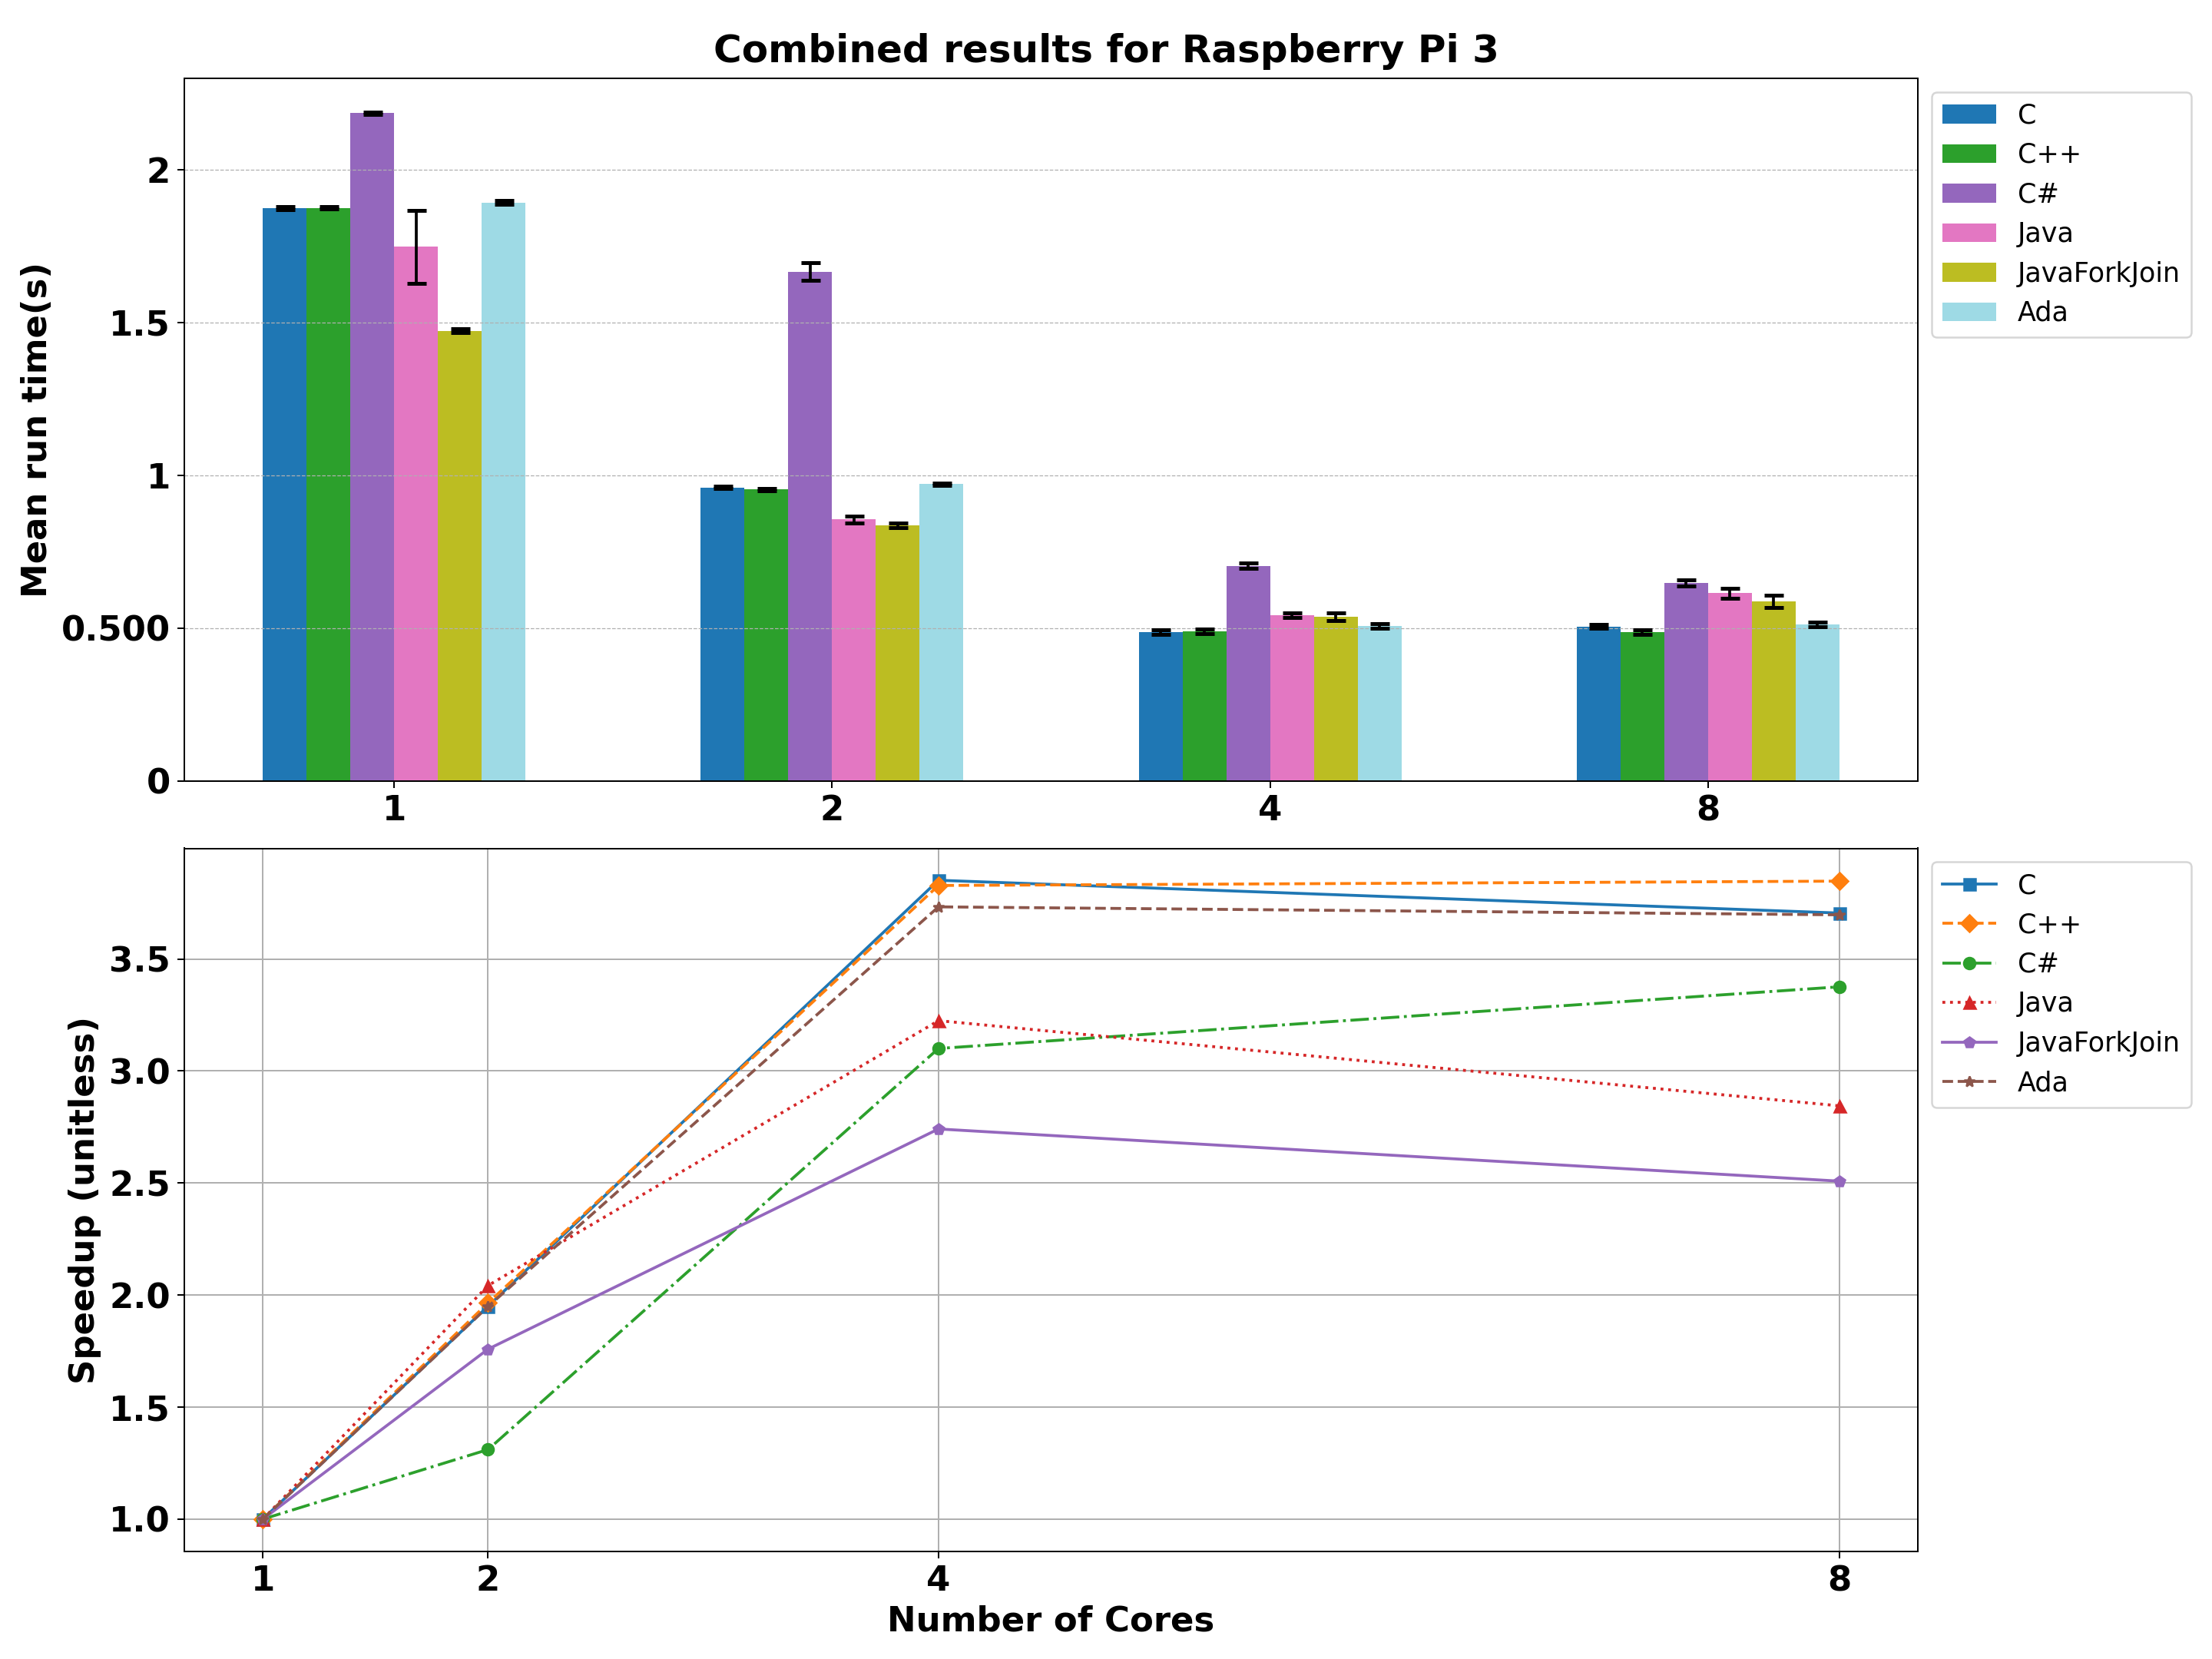
\includegraphics[width=1\textwidth, height=10cm]{~/Documents/Part_D_Modules/Individual_Project/Individual_report/figures/mpbenchmark_rpi3_results.png} % Adjust the path and width as needed
	\caption{Mean benchmark plot in seconds shown top. Speedup plot shown bottom.}
	\label{fig:mpbenchmark_rpi3_plot} % Use this label to reference the figure
\end{figure}

% Making the table fit in the page by scaling it down
\begin{table}[h!]
	\centering
	\resizebox{\textwidth}{!}{% Resizes the table to fit within the text width
		\begin{tabular}{|c|c|c|c|c|c|c|c|c|}
			\hline
			\textbf{Cores} & \textbf{C} & \textbf{C++} & \textbf{C++(NEON single)} & \textbf{C++(NEON double)} & \textbf{Java} & \textbf{JavaForkJoin} & \textbf{C\#} & \textbf{Ada} \\ \hline
			1              & 0           &0             & 0                         & 0                         &0               &0                     &0              &0             \\ \hline
			2              & 0          & 0             &  0                        &  0                         & 0.18         &0                     &0              &0             \\ \hline
			4              & 0           & 0            & 0                         & 0                          &1.33          &0                     & 0             &0             \\ \hline
			8              & 0           & 0            &  0                        &   0                        & 8.21         & 1.03               &0              &0             \\ \hline
		\end{tabular}
	}
	\caption{Mean deadlines missed, results collected from the Raspberry Pi 5.}
	\label{tab:mpbenchmark_rpi5} % Label for referencing
\end{table}

% Making the table fit in the page by scaling it down
\begin{table}[h!]
	\centering
	\resizebox{\textwidth}{!}{% Resizes the table to fit within the text width
		\begin{tabular}{|c|c|c|c|c|c|c|c|c|}
			\hline
			\textbf{Cores} & \textbf{C} & \textbf{C++} & \textbf{C++(NEON single)} & \textbf{C++(NEON double)} & \textbf{Java} & \textbf{JavaForkJoin} & \textbf{C\#} & \textbf{Ada} \\ \hline
			1              & 0           &0              &  0                          & 0                         &0.90              &0                      &0             &0             \\ \hline
			2              & 0          & 0              &  0                         &  0                         &1.00              &0.27                 &0             &0             \\ \hline
			4              & 0.005   & 0              &  0                         & 0.005                   &1.34              &0.52                 &0             &0.01             \\ \hline
			8              & 0.03      & 0.0295    &  0                         &  0.04                    &6.35             & 6.93                 &2.33        &0.04             \\ \hline
		\end{tabular}
	}
	\caption{Mean deadlines missed, results collected from the Raspberry Pi 4.}
	\label{tab:mpbenchmark_rpi4} % Label for referencing
\end{table}

% Setting the table with specified font size, without dynamic resizing
\begin{table}[h!]
	\centering
	{\fontsize{12pt}{12pt}\selectfont % Set font size to 10pt with a 12pt line spacing
		\begin{tabular}{|c|c|c|c|c|c|c|}
			\hline
			\textbf{Cores} & \textbf{C} & \textbf{C++} & \textbf{Java} & \textbf{JavaForkJoin} & \textbf{C\#} & \textbf{Ada} \\ \hline
			1              & 1.17       & 1.30         & 1.60          & 1.10                 & 3.40         & 1.33         \\ \hline
			2              & 2.80       & 2.47         & 2.73          & 2.40                 & 31.63        & 2.97         \\ \hline
			4              & 3.61       & 3.67         & 5.13          & 4.65                 & 19.33        & 3.83         \\ \hline
			8              & 44.60      & 46.55        & 30.2          & 25.23                & 46.63        & 43.57        \\ \hline
		\end{tabular}
	}
	\caption{Mean deadlines missed, results collected from the Raspberry Pi 3.}
	\label{tab:mpbenchmark_rpi3} % Label for referencing
\end{table}




\newpage
\section{Appendix (Objective 2: \texttt{MobileNet})}

The \texttt{MobileNet} repository\cite{mobilenet_repo} contained some outdated portions of the code which were updated, certain parts of the code contained Chinese language which were translated into English and \texttt{CMake} build software was used to setup the \texttt{MobileNet} application. 

The main updates required to the original \texttt{MobileNet} repository\cite{mobilenet_repo} were inside the \texttt{readdata.cpp} file (listing ~\ref{lst:mobilenet_updates}). 

\begin{lstlisting}[
	caption={Updating the \texttt{ReadData::ReadInput()} function to use the latest \texttt{OpenCV} functions.},
	label={lst:mobilenet_updates}
	]
float* ReadData::ReadInput(const char* pcName) {
	std::cout << "Reading Picture: " << pcName << "..." << std::endl;
	
	// Use cv::Mat for image representation
	cv::Mat srcImage = cv::imread(pcName, cv::IMREAD_UNCHANGED);
	if (srcImage.empty()) {
		std::cerr << "Error: Image not loaded." << std::endl;
		return nullptr;
	}
	
	// Resize image
	cv::Mat dstImage;
	cv::resize(srcImage, dstImage, cv::Size(m_nInputWidth, m_nInputHeight), 0, 0, cv::INTER_LINEAR);
	
	int nOutputIndex = 0;
	
	for (int i = 0; i < dstImage.rows; i++) {
		for (int j = 0; j < dstImage.cols; j++) {
			nOutputIndex = i * m_nInputWidth + j;
			cv::Vec3b pixel = dstImage.at<cv::Vec3b>(i, j);
			m_pfInputData[nOutputIndex] = static_cast<float>(pixel[0]) - m_pfMean[nOutputIndex];
			m_pfInputData[nOutputIndex + m_nImageSize] = static_cast<float>(pixel[1]) - m_pfMean[nOutputIndex + m_nImageSize];
			m_pfInputData[nOutputIndex + 2 * m_nImageSize] = static_cast<float>(pixel[2]) - m_pfMean[nOutputIndex + 2 * m_nImageSize];
		}
	}
	
	std::cout << "Reading Picture Done..." << std::endl;
	
	return m_pfInputData;
}
\end{lstlisting}

Figure ~\ref{fig:mobilenet_classes} shows the translation from Chinese to English language. The classes that the \texttt{MobileNet} was trained on were in Chinese therefore it was translated into English, found inside the \texttt{Network.cpp} file of the original project\cite{mobilenet_repo}. 

\begin{figure}[H] % Positioning preference: here, top, bottom, page
	\centering
	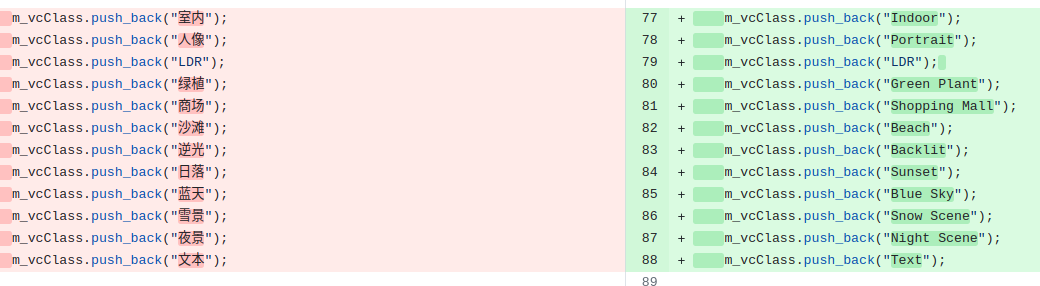
\includegraphics[width=1\textwidth, height=20cm]{~/Documents/Part_D_Modules/Individual_Project/Individual_report/figures/mobilenet_classes.png} % Adjust the path and width as needed
	\caption{\texttt{GitHub} page showing the commit diff when classes were translated from Chinese to English. }
	\label{fig:mobilenet_classes} % Use this label to reference the figure
\end{figure}

The application was modified to have three command line arguments, this served primarily to make testing and collecting benchmark results easier for development purposes. The three arguments are as follows and can be seen in code in listing ~\ref{lst:mobilenet_command_line_arguments}:

\begin{enumerate}
	\item \texttt{test\_all}: This argument can be altered to either test one image or test all images in the data folder.  
	\item \texttt{write\_to\_file}: This argument is for writing benchmark data to a \texttt{.txt} file, this was useful for development purposes. It is recommended to leave this blank, so the project does not save any benchmark data. 
	\item \texttt{threads}: The number of threads that will be used by the application. It can be left blank to use the maximum number of available threads.  
\end{enumerate}

\begin{lstlisting}[
	caption={Altering the \texttt{MobileNet} application to use three command line arguments. \texttt{./mobilenet [test\_all] [write\_to\_file] [threads]}},
	label={lst:mobilenet_command_line_arguments}
	]
	int main(int argc, char* argv[])
	{
		//---------------------------Command line app logic
		bool testAllImages = false;
		bool writeDataToFile = false;  // Declare the variable to handle write to file logic
		bool g_DebugMode = true;       // Default debug mode setting
		int numThreads = 1;            // Default to 1 thread unless specified
		
		if (argc > 1) {
			std::string firstArg(argv[1]);
			testAllImages = (firstArg == "test_all");
		}
		if (argc > 2) {
			std::string secondArg(argv[2]);
			writeDataToFile = (secondArg == "write_to_file");
			g_DebugMode = !writeDataToFile; 
		}
		if (argc > 3) {
			numThreads = std::atoi(argv[3]);
			if (numThreads <= 0) {
				numThreads = omp_get_max_threads();  
			}
		}
		//--------------------------------------------------
		// Further logic and operations can follow here
	}
\end{lstlisting}


\texttt{Calgrind} profiling results from the \texttt{MobileNet} application show the following functions with the highest self-cost, these were \texttt{ConvLayer::forward()}, \texttt{BatchNormalLayer::forward()} and \texttt{ConvLayer::Addpad()} as seen in figure ~\ref{fig:mobilenet_profiling}.

\begin{figure}[H] % Positioning preference: here, top, bottom, page
	\centering
	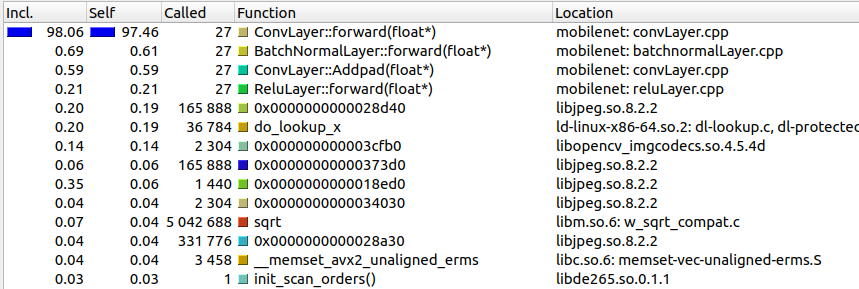
\includegraphics[width=1\textwidth, height=20cm]{~/Documents/Part_D_Modules/Individual_Project/Individual_report/figures/mobilenet_profiling.png} % Adjust the path and width as needed
	\caption{\texttt{Calgrind} profiling results, functions with the highest self-cost.}
	\label{fig:mobilenet_profiling} % Use this label to reference the figure
\end{figure}


The parallelisation of functions \texttt{BatchNormalLayer::forward()} and \texttt{ConvLayer::Addpad()} can be found in listings ~\ref{lst:mobilenet_function1_parallel} and ~\ref{lst:mobilenet_function2_parallel}.

\begin{lstlisting}[
	caption={Parallelising the \texttt{BatchNormalLayer::forward()} function.},
	label={lst:mobilenet_function1_parallel}
	]
void BatchNormalLayer::forward(float *pfInput) 
{
	#pragma omp parallel for collapse(2) shared(m_nInputNum, m_nInputSize, pfInput, m_pfOutput, m_pfFiller, m_pfMean, m_pfVar, m_pfBias) 
	for (int i = 0; i < m_nInputNum; i++)
	{
		for (int j = 0; j < m_nInputSize; j++)
		{
			int nOutputIndex = i * m_nInputSize + j;
			
			m_pfOutput[nOutputIndex] = m_pfFiller[i] * ((pfInput[nOutputIndex] - m_pfMean[i])
			/ sqrt(m_pfVar[i] + 1e-5)) + m_pfBias[i];
		}
	}
}
\end{lstlisting}


\begin{lstlisting}[
	caption={Parallelising the \texttt{ConvLayer::Addpad()} function If the \texttt{EMBEDDED\_PROC} is not set.},
	label={lst:mobilenet_function2_parallel}
	]
void ConvLayer::Addpad(float *pfInput)
{
	// Only use OpenMP pragmas if EMBEDDED_PROC is not defined, such as on a laptop/desktop CPU 
	#ifndef EMBEDDED_PROC
	#pragma omp parallel for collapse(2)
	#endif
	for (int m = 0; m < m_nInputNum; m++)
	{
		for (int i = 0; i < m_nInputPadWidth; i++)
		{
			for (int j = 0; j < m_nInputPadWidth; j++)
			{
				if ((i < m_nPad) || (i >= m_nInputPadWidth - m_nPad))
				{
					m_pfInputPad[m * m_nInputPadSize + i * m_nInputPadWidth + j] = 0;
				}
				else if ((j < m_nPad) || (j >= m_nInputPadWidth - m_nPad))
				{
					m_pfInputPad[m * m_nInputPadSize + i * m_nInputPadWidth + j] = 0;
				}
				else
				{
					m_pfInputPad[m * m_nInputPadSize + i * m_nInputPadWidth + j] = pfInput[m * m_nInputSize + (i - m_nPad) * m_nInputWidth + (j - m_nPad)];
				}
			}
		}
	}
}
\end{lstlisting}

% Addition of command line arguments
% Valgrind results 
% All the parallelised code
\newpage
\section{Appendix (Objective 3: \texttt{DeBaTE-FI} platform)}
\label{sec:app_obj3}

The application was profiled using \texttt{py-spy} tool. The application spawned multiple processes, therefore they were profiled separately. Profiling results from the process responsible for the GUI of the application are shown in figure ~\ref{fig:debate_profile_1} and the profiling results from the process responsible for communicating with the MCUs are shown in figure ~\ref{fig:debate_profile_2}.

\begin{figure}[H] % Positioning preference: here, top, bottom, page
	\centering
	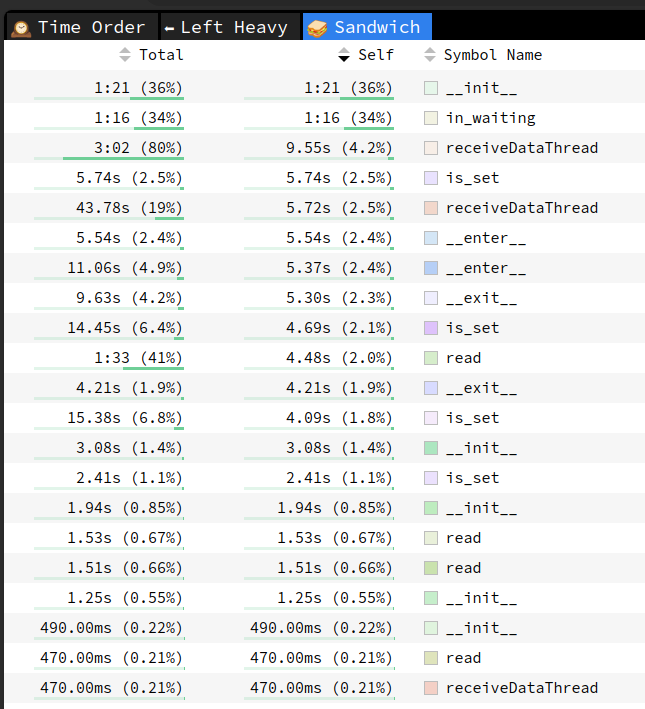
\includegraphics[width=1\textwidth, height=20cm]{~/Documents/Part_D_Modules/Individual_Project/Individual_report/figures/debate_fi_platform_app.png} % Adjust the path and width as needed
	\caption{Profiling results for the application GUI process visualised in \texttt{speedscope} web application\cite{speedscope_app}. }
	\label{fig:debate_profile_1} % Use this label to reference the figure
\end{figure}

\begin{figure}[H] % Positioning preference: here, top, bottom, page
	\centering
	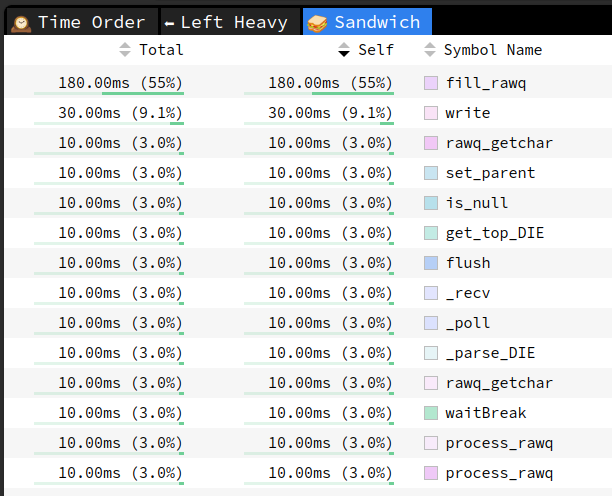
\includegraphics[width=1\textwidth, height=20cm]{~/Documents/Part_D_Modules/Individual_Project/Individual_report/figures/debate_fi_platform_openocd.png} % Adjust the path and width as needed
	\caption{Profiling results for the \texttt{OpenOCD/telnet} process visualised in \texttt{speedscope} web application\cite{speedscope_app}.}
	\label{fig:debate_profile_2} % Use this label to reference the figure
\end{figure}

Figure ~\ref{fig:debate_fi_telnetlibcpp} shows the thought process of designing the \texttt{C++} wrapper class to use the necessary \texttt{telnet} library for \texttt{DeBaTE-FI} platform. 

\begin{figure}[H] % Positioning preference: here, top, bottom, page
	\centering
	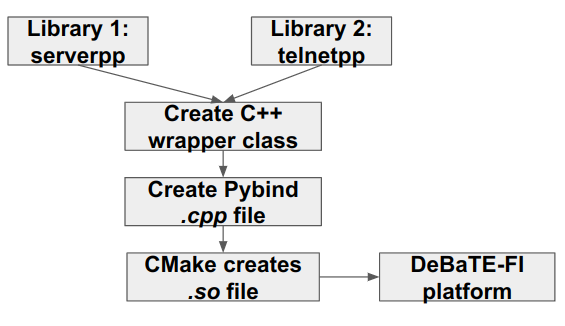
\includegraphics[width=0.50\textwidth]{~/Documents/Part_D_Modules/Individual_Project/Individual_report/figures/debate_fi_C++_design.png} % Adjust the path and width as needed
	\caption{Design process for creating the \texttt{telnet} library using \texttt{C++}.}
	\label{fig:debate_fi_telnetlibcpp} % Use this label to reference the figure
\end{figure}

The \texttt{C++} wrapper was created by emulating the \texttt{Python's} \texttt{telnetlib} library.Using the code in listing ~\ref{lst:open_ocd_class} the following functions require emulation:

\begin{enumerate}
	\item \texttt{read\_some()}
	\item \texttt{write()}
	\item \texttt{Exec()}
	\item \texttt{Readout()}
\end{enumerate}


\begin{lstlisting}[
	caption={Functions used from \texttt{Python's} \texttt{telnetlib} library.},
	label={lst:open_ocd_class}
	]
import telnetlib

class OpenOCD:
	def __init__(self, Host="localhost", Port=4444):
		try:
			self.tn = telnetlib.Telnet(Host, Port)
		except ConnectionRefusedError as e:
			print("ERROR: Could not open port",Port)
			raise e
		self.Readout()

#
# Communication functions
#
	def Readout(self):
		s = ''
		Lines = []
		while True:
			s += self.tn.read_some().decode('UTF-8') # 'telnetlib' function called
			l = s.splitlines()
		if len(l) > 1:
			for s in l[:-1]:
				if len(s) > 0:
					Lines.append(s)
			s = l[-1]
	if s == '> ':
		return Lines

	def Exec(self, Cmd, *args):
		Text = Cmd
		for arg in args:
			if arg:
				Text += ' ' + arg
		Text += '\n'
		self.tn.write(bytearray(Text, 'UTF-8')) # 'telnetlib' function called
		return self.Readout()
\end{lstlisting}

Using the open-source \texttt{telnet} libraries in \texttt{C++}: \texttt{telnetpp}\cite{telnetpp_library} and \texttt{serverpp}\cite{serverpp_library} the necessary functions were created in the wrapper class seen in figure ~\ref{fig:telnetlibcpp_UML}. Listing ~\ref{lst:c++_telnetlibcpp} shows the code:

\begin{lstlisting}[
	caption={\texttt{C++} wrapper class to integrate with the \texttt{Python} application. Emulating functions \texttt{read\_some()}, \texttt{write()}, \texttt{Exec()} and \texttt{Readout()}. },
	label={lst:c++_telnetlibcpp}
	]
std::vector<serverpp::byte> TelnetlibCpp::read_some() {
	incoming_data_ = false; // Ensure the flag is reset before starting the async operation
	receivedData_.clear(); // Clear previous data
	// Return a copy of the data or move receivedData as appropriate
	telnet_session_.async_read([this](gsl::span<const serverpp::byte> data) {
		if (!data.empty()) {
			// Directly assign the data since receivedData is a member variable
			receivedData_.assign(data.begin(), data.end());
		}
		incoming_data_ = true; // Indicate that data has been received or the operation is complete
	});
	// Efficiently wait for the async operation to complete using io_context.run_one()
	while (!incoming_data_) {
		io_context_.run_one();
	}
	// Return a copy of the data or move receivedData as appropriate
	return receivedData_;
}

void TelnetlibCpp::write(const std::vector<serverpp::byte>& data) {
	// Assuming 'serverpp::byte' is compatible with 'telnetpp::byte'
	// Wrap the data in a 'telnetpp::bytes' variant to create a 'telnetpp::element'
	telnetpp::bytes byte_data(data.data(), data.size());
	telnetpp::element elem = byte_data;  // Implicitly converts to variant
	
	// Now call the write method with the constructed element
	telnet_session_.write(elem);
}

std::vector<std::string> TelnetlibCpp::Exec(const std::string& cmd, const std::vector<std::string>& args) {
	std::string text = cmd;
	for (const auto& arg : args) {
		if (!arg.empty()) {
			text += ' ' + arg;
		}
	}
	text += '\n';
	
	// write(Cmd), write directly to avoid unnecessary conversions 
	telnetpp::bytes byte_data(reinterpret_cast<const std::uint8_t*>(text.data()), text.size());
	telnetpp::element elem = byte_data;
	telnet_session_.write(elem); 
	//-----------------------------------------------------------------------------------------
	
	// Read and return the output
	return Readout();
}

std::vector<std::string> TelnetlibCpp::Readout() {
	std::string s;
	std::vector<std::string> lines;
	
	while (true) {
		std::vector<std::uint8_t> byte_data = read_some();
		std::string chunk(byte_data.begin(), byte_data.end());
		
		s += chunk;
		
		size_t start_pos = 0;
		size_t pos;
		while ((pos = s.find('\n', start_pos)) != std::string::npos) {
			if (pos > start_pos) { // Ignore empty lines
				std::string line(s.begin() + start_pos, s.begin() + pos);
				line.erase(std::remove(line.begin(), line.end(), '\r'), line.end());
				line.erase(std::remove(line.begin(), line.end(), '\x00'), line.end());
				
				if (line.size())
				lines.push_back(std::move(line)); // Use move semantics to avoid copying
			}
			start_pos = pos + 1;
		}
		s.erase(s.begin(), s.begin() + start_pos); // Only erase the processed part
		
		if (s.find('>') != std::string::npos) {
			return lines; // Assuming lines are already filtered correctly
		}
	}
}

\end{lstlisting}

This was integrated into the \texttt{Python} application using a tool called \texttt{pybind11}. This required creating a \texttt{.cpp} file to allow the \texttt{C++} funtions to be called from the \texttt{Python} file, this is seen in listing ~\ref{lst:pybind_c++_file}.

\begin{lstlisting}[
	caption={Preparing our \texttt{C++} class \texttt{telnetlibcpp} using \texttt{pybind11} to be used with \texttt{Python}.},
	label={lst:pybind_c++_file}
	]
#include <pybind11/pybind11.h>
#include <pybind11/stl.h> // For automatic conversion of std::vector
#include "telnetlibcpp.hpp" // Include your class definition

namespace py = pybind11;

PYBIND11_MODULE(telnetlibcpp, m) {
	py::class_<TelnetlibCpp>(m, "TelnetlibCpp")
	.def(py::init<const std::string&, serverpp::port_identifier>())
	.def("Readout", &TelnetlibCpp::Readout) // Bind the Readout function
	// Bind the Exec function, using a lambda to handle optional vector<string> args
	.def("Exec", [](TelnetlibCpp& self, const std::string& cmd, const py::list& args) {
		std::vector<std::string> vecArgs;
		for (const auto& arg : args) {
			if (!arg.is_none()) {
				vecArgs.push_back(arg.cast<std::string>());
			} else {
				// Optionally, handle None values differently, e.g., by inserting an empty string
				// vecArgs.push_back("");
			}
		}
		return self.Exec(cmd, vecArgs);
	})
	.def("read_some", &TelnetlibCpp::read_some)
	.def("write", &TelnetlibCpp::write)
	.def("write_raw_sequence", &TelnetlibCpp::write_raw_sequence)
	.def("run", &TelnetlibCpp::run);
}
\end{lstlisting}

The final step was to compile the \texttt{C++} codes into a shared library(\texttt{.so}) file which was then placed in the directory of the \texttt{Python} application where it needed to be used. Listing ~\ref{lst:cmake_so_file} shows hows this shared library file was created. 

\begin{lstlisting}[
	caption={\texttt{CMake} file to produce a shared library(\texttt{.so}) file of the \texttt{C++} class.},
	label={lst:cmake_so_file}
	]
cmake_minimum_required(VERSION 3.14 FATAL_ERROR)
project(telnetlibcpp)

# Set the C++ standard
set(CMAKE_CXX_STANDARD 17)
set(CMAKE_CXX_STANDARD_REQUIRED ON)
set(CMAKE_EXPORT_COMPILE_COMMANDS ON)

# Optimization flag -O3 for Release builds
set(CMAKE_CXX_FLAGS_RELEASE "-O3")

# Include Pybind11
include(FetchContent)
FetchContent_Declare(
pybind11
GIT_REPOSITORY https://github.com/pybind/pybind11.git
GIT_TAG v2.6.1
)
FetchContent_MakeAvailable(pybind11)

# Find required Boost components in one call
find_package(Boost REQUIRED COMPONENTS container locale)
find_package(serverpp REQUIRED)
find_package(telnetpp 3.0.0 REQUIRED)
find_package(gsl-lite REQUIRED)

# Source files including the Pybind11 binding file
set(SOURCE_FILES
src/telnetlibcpp.cpp
src/pybind_module.cpp  # Your Pybind11 binding source file
)

# Compile as a shared library
add_library(telnetlibcpp SHARED ${SOURCE_FILES})

target_include_directories(telnetlibcpp PRIVATE include)

target_link_libraries(telnetlibcpp
PRIVATE
KazDragon::serverpp
KazDragon::telnetpp
Boost::container
Boost::locale
pybind11::module  # Link against Pybind11 module support
)

# Set output library name and ensure it doesn't have the 'lib' prefix
set_target_properties(telnetlibcpp PROPERTIES PREFIX "" OUTPUT_NAME "telnetlibcpp")
\end{lstlisting}


